\chapter{Background}
\label{chp:background} 

\section{Village Telco}
%How did it all start?


\section{Mesh Potato}

The Village Telco concept was developed in June 2008 during a workshop at the Shuttleworth Foundation. The main goal was to figure out how to develop an inexpensive system to provide rural and under-served areas with affordable telephone communication \cite{MParticle}. The workshop included participants like open hardware pioneer Dawid Rowe, and Elektra, the developer of B.A.T.M.A.N. \cite{MPworkshop}. The purpose of the workshop was to develop a business model, as well as a prototype for a Village Telco. Initially the idea was to use low cost VoIP headsets. At that time it was the most viable and convenient way to deliver telephone services to the customers. The wireless VoIP telephones have small antennas, which became a problem. The nodes could not be more than 100 meters away from each other in order to have a reliable connection. This  required more nodes in order to cover the desirable area. This factor drastically increased the start-up costs for a village. In order to keep the cost down, it was also important to keep the number of access points (APs) down. A mesh network has a larger range, and one suggestion was to use a small mesh device like an Open Mesh AP and connect a SIP phone to it. This solution would solve a lot of the problems regarding range, antenna and number of access points, but the idea was still an expensive option. The challenge was to create something that would be simple enough to be configured and scaled by local entrepreneurs with limited technical skills. In addition to this it was important to keep the cost down. The two key cost factors that emerged in the scale-up of a Village Telco were the cost of the customer's phone and the power supply. It was clear that the power supply was the most important factor, and that they had to look at other, and cheaper options regarding the customers phones \cite{MPworkshop}. During the debating, Rael Lissoos took an Analogue Telephone Adapter (ATA) and an Open Mesh AP, held them together and said \textit{"we need these two devices in one"}. This point was the birth of the Mesh Potato, fully based on customized open hardware and open software design. The name "Mesh Potato" comes from combining the words mesh, POTS (Plain Old Telephone) and ATA. "Patata" is the Spanish word for potato, and hence the name Mesh Potato. The Mesh Potato is a mesh enabled Wi-Fi device, with the possibility to connect any inexpensive regular phone and IP device. \cite{MPorigin}

\begin{figure}[b]
  \centering
      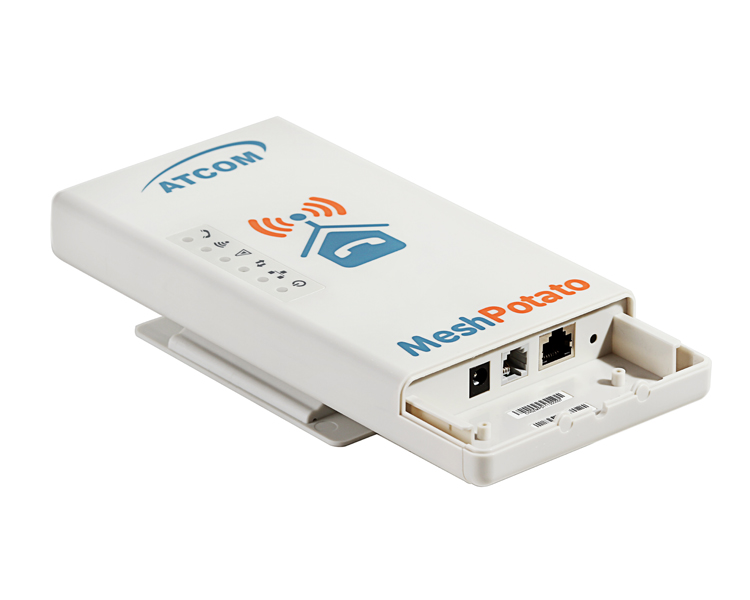
\includegraphics[width=0.5\textwidth]{MP01}
  \caption [MP01]{\textbf{The first generation Mesh Potato, MP01.}}
  \label{fig:MP01}
\end{figure}

The first generation of the Mesh Potato is shown in \fref{fig:MP01}. This device is designed to be used in rural areas. It can be deployed and run anywhere in the world, relying only on a low, but stable, power supply. The Ethernet port, the Foreign eXchange Station (FXS) ports and the power port are robust and designed in order to handle all weather conditions, poor power conditions, lightening and static electricity. In addition to this, the Mesh Potato comes in a waterproof box for outdoor mounting \cite{background}.

The Mesh Potato combines the features of a 802.11bg Wi-Fi router with an Analogue Telephone Adaptor (ATA) \cite{MP}. The ATA converts the signal from a standard telephone, into the digital signal needed to connect to the Internet and use the SIP protocol \cite{MParticle}. The device is based on the Atheros chipset that is used by OpenMesh, and runs OpenWrt (see section \ref{subsec:openwrt} for more information) and B.A.T.M.A.N. (see section \ref{subsec:batman} for more information). Each Mesh Potato provides a single fixed telephone line to the end user. The MPs are connected together via a mesh Wi-Fi network, and configure themselves automatically to form a peer-to-peer network, greatly extending the range of the network over regular Wi-Fi. This enables the phone calls to be made independent of landlines and telephone towers, and creates the basis for the "plug-and-play" solution. 

As mentioned, the Mesh Potato is open and based on open hardware, as well as open software design. Everything is kept open in order for any third party to test, set standards, and give feedback. Key goals during the development was to minimize the binary blobs (a closed source binary-only driver that has no publicly available source code \cite{binaryBolb}), minimize closed software and make the hardware open. 

The mesh network can be connected via a backbone link to the rest of the world by using VoIP gateways. No cell phone towers, no land lines, and no telecommunication companies are required. A Village Telco is a community owned telephone service, allowing a local entrepreneur to roll out the Village Telco system only needing a server and the wanted amount of Mesh Potatoes. The mesh network is self-healing and self-organizing, meaning if one node goes down, B.A.T.M.A.N. routes the calls through other available nodes in the network \cite{MPbyRowe}. In order to provide internet access, a super node has to be placed in connection with an internet connection. The internet signal enters the server in the Village Telco, this could for example be an existing internet café, with a broadband, link or satellite connection. The signal is transmitted to the super node. The super node consists of three external access points, and is placed high over ground, giving 360 degree coverage, with approximately 1 km range. The internet signal is then carried through the network from one Mesh Potato to another. 


\subsubsection{Mesh Potato 2.0}
The first generation of the Mesh Potato has sold over 2500 copies, and is deployed all over the world. In order to keep up with time, the constant technical development and the demand from the users, a new version of the Mesh Potato was introduced. The second generation became available to users August 2013. This device comes in a smaller box, as shown in \fref{fig:MP02}, and is sold to half the price of the first generation. One of the biggest differences is that the second generation has two Ethernet ports and is built on a new, and faster, chipset. It is also  operating on new firmware.

\begin{figure}[h!]
  \centering
      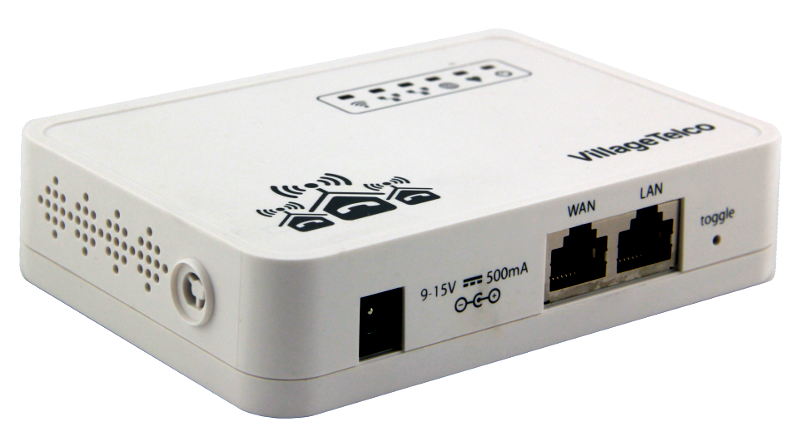
\includegraphics[width=0.5\textwidth]{mp2.PNG}
  \caption [MP2]{\textbf{The second generation Mesh Potato, MP2.}}
  \label{fig:MP02}
\end{figure}

\subsubsection{Difference between MP01 and MP02?}



\subsubsection{Example Mesh network}
\begin{figure}[b]
  \centering
      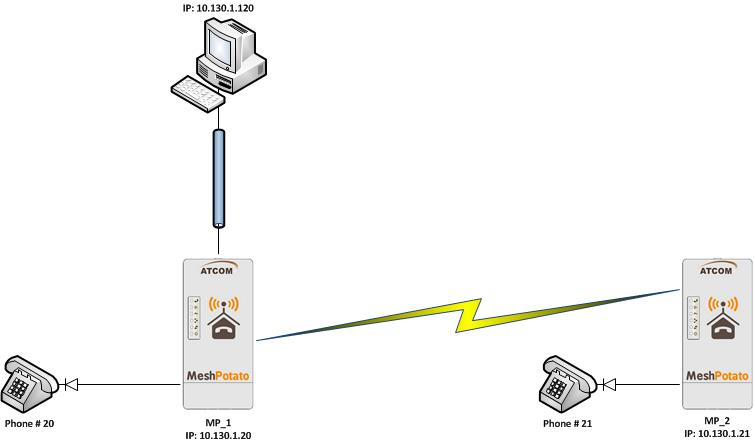
\includegraphics[width=1\textwidth]{network1}
  \caption [Example of a simple mesh network]{\textbf{Simple mesh network.} This figure illustrates a simple mesh network with the use of Mesh Potatoes.}
  \label{fig:network}
\end{figure}

An example of how to set up a simple network is shown in \fref{fig:network}. The network consists of two regular telephones connected to each their Mesh Potato. The MP devices has been assigned static IP addresses, these addresses are not part of the LAN address space. The IP addresses are allocated in a predefined default address space 10.130.1.xxx. To administrate the MP devices one can use a workstation linked together with any of the MPs in the network (either by using a Ethernet cable or Wi-Fi). This workstation must be assigned a static address within the same address space as the MP devices. Phone calls may be done between the Mesh Potatoes by dialling the last octet or the whole IP address. See the user guide in Appendix for a more detailed description of how to set up the Mesh Potatoes and how different networks can be built. 


\section{Relevant Technologies}
In this section we will go through some of the most relevant technologies used to develop and run the Mesh Potatoes. In order to understand how the Mesh Potato works, it is important to have a certain knowledge about the underlying technology. 

\subsection{OpenWrt}
\label{subsec:openwrt}
OpenWrt is an embedded open-source operating system for routers distributed by Linux \cite{openwrt}. It is extensible and can easily be modified to suit any application, since it offers a file system with a package manager. OpenWrt provides (1) Free and open-source, (2) Easy and free access, and are (3) Community Driven \cite{openwrt}. This means that the source code is free and available to everyone, and that everyone has the opportunity to contribute to it. 

\subsection{Mobile Ad Hoc Networks}

\begin{figure}[b]
  \centering
    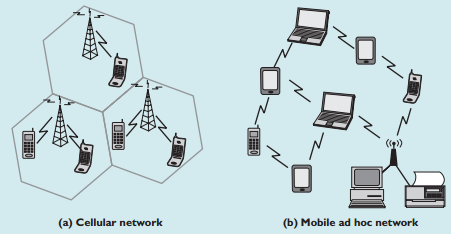
\includegraphics[width=0.8\textwidth]{adhoc.png}
     \caption [Cellular network vs. MANET]{\textbf{Cellular network vs. MANET}. This figure illustrates the difference between a regular cellular network and a mobile ad hoc network \cite{adhoc2}.}
\label{fig:adhoc}
\end{figure}

Mobile ad hoc networks (MANETs) are networks that do not rely on an underlying and fixed infrastructure (access points and routers), in other words "infrastructure-less". MANETs acts in a shared wireless media \cite{adhoc}. The structure of these networks change dynamically, and key factors describing MANETs is self-configuration, self-organization, self-discovery, and self-healing \cite{wmn}. The members of the network are mobile and are free to join or leave the network at any time \cite{adhoc2}, and therefore these factors are important. MANETs are based on multi-hop forwarding. Each node acts not only as a host, but also as a router. The nodes themselves establish and maintain routes, and forward packets to other nodes if necessary. This enables communication between nodes that are originally not within each other's range \cite{adhoc2}. MANETs are suited for use in situations where there is no fixed underlying infrastructure. A MANET can operate as a stand-alone solution, but can also be attached to the Internet. This makes room for numerous of services. 

\begin{figure}[b]
  \centering
    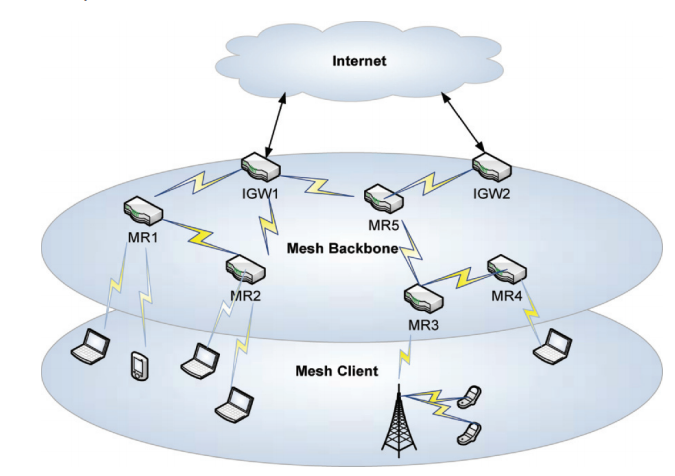
\includegraphics[width=0.8\textwidth]{wmn.png}
     \caption [Example of a Wireless Mesh Network]{\textbf{Example of a Wireless Mesh Network}. This figure illustrates the architecture of a typical WMN \cite{wmn}.}
\label{fig:wmn}
\end{figure}

\subsection{Wireless Mesh Networks}
A wireless mesh network (WMN) is a type of MANET \cite{wmn}. The objective of a WMN is to serve a larger number of users with high bandwidth access. As mentioned before, MANETs are "infrastructure-less" and they have self-configuration, self-organizing, self-healing and self-discovering features. WMNs share all these characteristics, except from the infrastructure part. WMNs, on the contrary to MANETs, are often a collection of routers called mesh routers (MRs). These MRs are usually stationary. The MRs can be employed for different use. One MR could for example be connected via cable to Internet, and then become a Internet gateway. Then this MR can provide Internet connectivity to the other MRs in the mesh network. A wireless mesh network consists of two parts \cite{wmn}; the backbone of the mesh (the MRs) and the clients of the mesh. An example of a WMN architecture is shown in \fref{fig:wmn}. 


\subsection{Routing Protocols}
Ad hoc networks and mesh networks creates several challenges when it comes to routing protocols. The routing protocols must be able to adapt quickly due to the topology changes. \fref{fig:adhocprotocols} shows the different groups of the ad hoc protocols that exist. It is important that a routing protocol do not cause excessive overhead (extensive use of computer resources). Under the category flat routing, there are two types of routing protocols; proactive and reactive. \textit{Proactive routing protocols} (e.g. OLSR) are table driven \citep{proactivereactive}. Every network node has a routing table for the forwarding of data. To obtain stability, each node broadcasts and modifies the routing table periodically. Proactive routing protocols are suitable when there are few nodes in the network. The routing table is periodically updated, hence the overhead exceeds the desired value when there are a high number of nodes in the network. In contrary to the proactive routing protocols, \textit{reactive routing protocols} (e.g. AODV) are on demand. Since they are on demand, the overhead is significantly lower. These protocols utilize flooding. The network is flooded with the route request (RREQ) in order to set up the route. The reactive routing protocols do not have a up-to-date routing table like proactive routing protocols \cite{proactivereactive}. Routes are only set up to nodes they communicate with, and these routes are only kept alive while they are needed  \cite{adhoc2}. As shown in \fref{fig:adhocprotocols}, there are several different protocols under proactive and reactive. 


\begin{figure}[t]
  \centering
    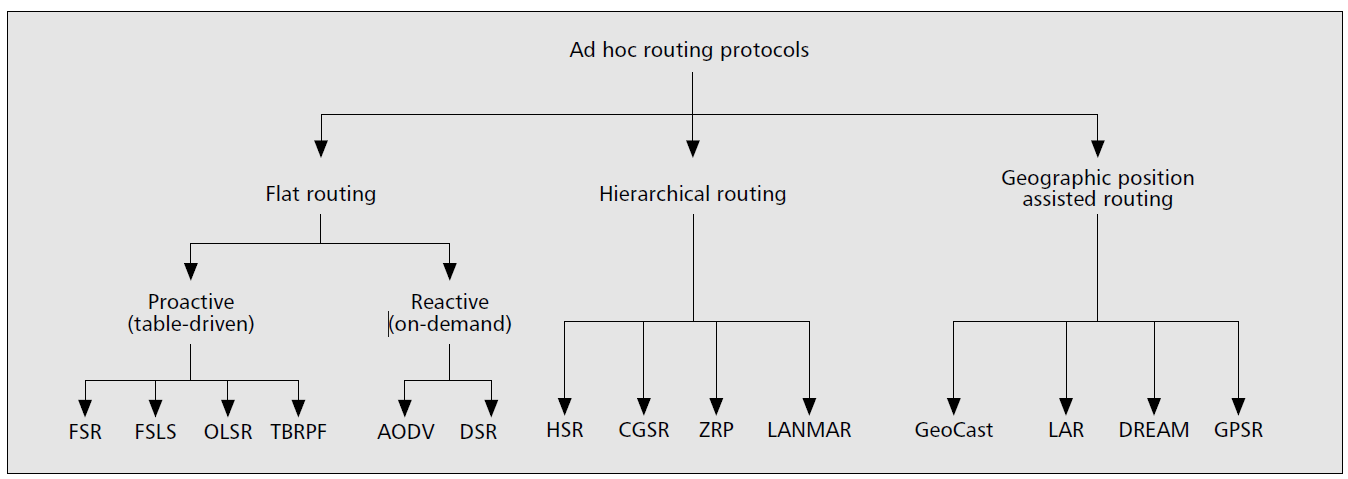
\includegraphics[width=1\textwidth]{adhocprotocols.png}
     \caption[Ad Hoc routing protocols]{\textbf{Different groups of ad hoc routing protocols \cite{adhoc}.}}
\label{fig:adhocprotocols}
\end{figure}


\subsection{B.A.T.M.A.N}
\label{subsec:batman}
Better Approach To Mobile Adhoc Networking (B.A.T.M.A.N) is the routing protocol utilized in the networks formed by the Mesh Potatoes. B.A.T.M.A.N is a proactive routing protocol for wireless ad hoc networks. This includes MANETs \cite{batman}. This protocol was developed as an alternative to OLSR (Optimized Link State Routing) \cite{batman2}. Like mentioned before, routing protocols must be able to adapt quickly to topology changes. B.A.T.M.A.N was made to be a more efficient routing protocol in this area, since it employs a new method for discovering routes. The nodes in the network broadcasts a OGM periodically, like shown in \fref{fig:batman}. A OGM is a Originator Message which contains: 

\begin{itemize}
\item The address of the node
\item Sequence number
\item TTL (Time to live)
\end{itemize}

The address and the sequence number enables identification of a packet and duplicate detection. 

\begin{figure}[b]
  \centering
    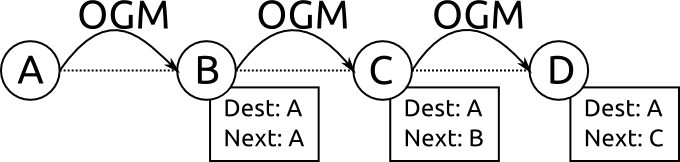
\includegraphics[width=0.8\textwidth]{batman.png}
     \caption[Originator Message in B.A.T.M.A.N]{\textbf{Originator Message used in B.A.T.M.A.N \cite{batman2}.}}
\label{fig:batman} 
\end{figure}


Information about the nodes that are accessible via single-hop or multi-hop are maintained and updated \cite{batman}. Every node updates its routing table each time it receives an OGM. The routing table includes information about \cite{batman2}:

\begin{itemize}
  \item \textbf{Originator Address:} This is the source address of the node that sent the OGM.
  \item \textbf{Current Sequence Number:} The sequence number of the last OGM. This is used to discover if there are any duplicates or any information that is outdated.
  \item \textbf{Sliding Window:} A list of sequence numbers that is stored for each originator and each previous hop, i.e. for the neighbour node that forwarded or originated the OGM, as shown in \fref{fig:batman}. This is used to decide which next hop is best for each destination. 
\end{itemize}

When a node receives an OGM it will decrease the TTL, and then forward it to the neighbour nodes. The same OGM can arrive to a node, but from different paths. In this case, only the first copy is preserved. 

\subsubsection{RO.B.IN}
RO.B.IN (Routing Batman Inside) uses the B.A.T.M.A.N routing algorithm. It is a project based on open source, and is intended for wireless mesh networks. It runs on Atheros AP51 routers running OpenWrt. RO.B.IN has the ability to spread wired internet (e.g. DSL) throughout a specific area, for example a village or a school \cite{robin}. 

\subsubsection{Simple Unified Dashboard for mesh networks}
Simple Unified Dashboard (SPUD) for mesh networks is a tool for visualization made for B.A.T.M.A.N mesh networks, and for the users of the networks \cite{spud}. The Simple Unified Dashboard is, like the name insinuates, a dashboard based on PHP which is designed to be simple. It communicates with the B.A.T.M.A.N visualization server. The dashboard makes it possible to monitor the link status of the networks, by displaying real time wireless link status. Other features are client management and customization. The software is written in CakePHP and for visualization SPUD uses Google Maps API 1.3 \cite{spud}.







\section{The Cost Structure and Revenue Model(s) of Village Telco Today}

\section{Comparison of Village Telco and other Telecommunication Companies}
